% Here, focus on the development of MGDO (waveform processing
% framework, data objects), OrcaROOT, and other tools 


\chapter{Analysis Tools}
\label{app:MGDO}

This appendix outlines several technical aspects related to the software work in this dissertation and can serve as a full or partial reference for the following:

	\begin{enumerate}
		\item \MJ~GERDA Data Objects (MGDO) -- software framework for encapsulation and processing of waveforms
		\item Analysis, Run database and processing framework
		\item pyWIMP, a software framework for generating limits on a WIMP signal
	\end{enumerate}

	\section{\MJ~GERDA Data Objects (MGDO)}
	\label{sec:WaveformProcMGDO}
	\lstset{
	   language=C++,
	   backgroundcolor=\color{lightgray},
	   extendedchars=true,
	   basicstyle=\footnotesize\ttfamily,
	   keywordstyle=\bfseries,
	   showstringspaces=false,
	   showspaces=false,
	   numbers=left,
	   numberstyle=\footnotesize,
	   numbersep=9pt,
	   tabsize=2,
	   breaklines=true,
	   showtabs=false,
	   captionpos=t}
	
	
	The \MJ~GERDA Data Objects (MGDO) \cpp-based software package has been
jointly developed by the \MJ~\cite{MJCollaboration} and
GERDA~\cite{GERDACollaboration} collaborations as a framework for
encapsulating and processing waveform data.  This section will reference some
of the functionality and layout of this software package, focusing on the
overall structure as well as particular aspects specifically relevant to this
dissertation.  This is meant to supplement the reference materials already
available, including a basic user and installation guide that ships with the
distribution.  MGDO is available on specific request to the \MJ~or GERDA
software groups at the following subversion
repository~\url{svn://pclg-soft.mppmu.mpg.de/MGDO}.  This section will outline
the basic structure and functionality of MGDO and then proceed to describe in
more detail the waveform transformations that ship with the software and have been developed
related to this dissertation work,
emphasizing aspects important for users rather than programmers of the package.  

		\subsection{Structure}
		
		The MGDO software is composed in the following package structure:

			\begin{enumerate}
				\item Base -- Base classes
				\item Root -- Root wrappers for base classes, allowing serialization of encapsulation classes and usage of calculation classes from ROOTCINT or pyROOT.
				\item Transforms -- Transform classes for objects performing a calculation or modification on a waveform
				\item Majorana -- \MJ-specific classes intended for encapsulation of data in the \MJ~data format
				\item Gerda -- GERDA-specific classes intended for encapsulation of data in the GERDA data format.
			\end{enumerate}
		Further description will focus only on the first three sub-packages and will leave the reference of objects particular to the \MJ~or GERDA collaborations to their respective owners or developers.
		
		\subsection{Base}
	This package includes base classes for all the objects within MGDO,
including encapsulation classes and others providing virtual interfaces for
derived.  The main encapsulation classes are as follows:

			\begin{enumerate}  
				\item[]{\lstinline!class MGWaveform!} Provides a
base encapsulation class for waveforms, storing e.g.~raw trace, sampling
information, type (charge, current, etc.) and providing access functions and
overloaded operators for simple calculations. 
				\item[]{\lstinline!class MGWaveformFT!} Provides a base
encapsulation class for frequency waveforms, and is specifically tailored to
hold data from the fast Fourier transform of real-data.  Provides similar
access and storage functionality to \lstinline!MGWaveform!. 
			\end{enumerate}  
The main virtual base classes are:
			\begin{enumerate}  
				\item[]{\lstinline!class MGVWFFastFourierTransform!}  Provides
a virtual interface for fast Fourier transform (FFT) classes.  Derived from
this class are particular implementations, including
\lstinline!MGWFFastFourierTransformDefault! and
\lstinline!MGWFFastFourierTransformFFTW! which provide a basic FFT and a
wrapped version of FFTW3~\cite{FFTW05}, respectively. 
				\item[]{\lstinline!class MGVWaveformTransformer!}  Provides a
virtual interface for generating waveform transformations or calculations, see
Section~\ref{sec:MGDOTransforms}.  \lstinline!class MGMultiWaveformTransformer!
provides a base class for chaining multiple waveform transformations together. 
				\item[]{\lstinline!class MGVFreqDomainTransformer!}  Provides
a virtual interface for generating transformations or calculations on a
waveform in frequency space, see Section~\ref{sec:MGDOTransforms}.  This base
class handles the necessary transformations to Fourier space.
\lstinline!class MGMultiFreqDomainTransformer! provides a base class for chaining
multiple frequency-domain transformations together. 

			\end{enumerate}  
		\subsection{Root}
			
	The Root sub-package includes objects that may depend on the ROOT analysis package.  In particular, this directory provides
wrapped code for Base class objects, enabling them to be serialized or loaded during a ROOT interactive session in ROOTCINT or pyROOT.  It also introduces a class: \lstinline! class MGTDataObject : public TNamed ! which provides an inheritance layer between ROOT objects and MGDO objects.  In general, every MGDO class requiring ROOT dependence should derive from this class.  Some base classes are merely wrapped:
			\begin{lstlisting}[label=lst:RootWrappedExamp]
...
class MGTVWaveformTransformer : public MGTDataObject, public MGVWaveformTransformer 
{
  public:
    MGTVWaveformTransformer(const std::string& aTransformationName);
    virtual ~MGTVWaveformTransformer();    
    virtual void Transform(MGWaveform* anInput, MGWaveform* anOutput = NULL) = 0;
    
  protected:
  ClassDef(MGTVWaveformTransformer, 0) 
};
...			\end{lstlisting}		
whereas others add some functionality, e.g.~\lstinline! class MGTWaveform !:
			\begin{lstlisting}[label=lst:RootWaveformExamp]
...
class MGTWaveform : public MGTDataObject, public MGWaveform
{
    ...
    // Returns a histogram named MGTWaveformHist_[label/ID]. If the user does not
    // supply an ID, the waveform ID is used. The function first searches
    // gROOT for MGTWaveformHist_[label/ID]. If it is found, that hist is used.
    // If it is not found, the function returns a newly allocated histogram 
    // of the waveform. Either way, it is the user's responsibility to
    // delete the histogram.
    virtual TH1D* GimmeHist(const char* label=""); 

    // Deprecated versions
    virtual TH1D* GetNewHist();
    virtual TH1D* GetNewHist(int id); 

    // When you don't care what the lable is and just want a brand-new,
    // unique histogram, call the following function
    virtual TH1D* GimmeUniqueHist(); 

    // Loads the waveform into a user-supplied hist. This function is safer
    // because it is obvious that the user owns (and therefore must later
    // delete) this histogram.
    virtual void LoadIntoHist(TH1D* hist);

    // Returns a TF1 object that is based on the       
    // loaded waveform.  There are three parameters for this TF1:
    //    parameters[0] - normalization (a)
    //    parameters[1] - constant factor (b)
    //    parameters[2] - offset (c)
    //    
    //   MGWaveform is a function of x == wf(x)
    // This function returns a TF1 with the underlying structure:
    //  a * wf( b*x + c )
    //  
    // Linear interpolation is applied when values are requested between 
    // data indices.
    //
    // iCopy specifies a different number of the function to return.
    // The name of the function takes the form:
    //
    // MGTWaveformFunction_[ID]_[Copy] 
    //
    // where ID is the id of the histogram and Copy is the passed in iCopy.
    // If this function already exists, it is deleted and  
    virtual TF1* GetFunction( int iCopy = 0 );

  protected:
    enum EWFFunctionPars { kNumberOfParameters = 3 }; 
    TF1* fWaveformFunction;
    double InterpolatingWaveformFunction( const double* x, 
                                          const double* parameters ); 

  ClassDef(MGTWaveform, 2) // Waveform class, holds waveforms
};

...			\end{lstlisting}		
which adds the capabilities of interpolation and export to 
other ROOT class formats (e.g.~\lstinline!TF1, TH1D!).
		\subsection{Transforms}
		\label{sec:MGDOTransforms}
		
	This package includes basic waveform transforms which are derived from \lstinline!class MGVWaveformTransformer!  and \lstinline!class MGVFreqDomainTransformer!, which define the basic interfaces for time-domain and  frequency-domain transformations, respectively.  The latter derives from the former.  The use of the transformations involves calling the class function
\lstinline! virtual void MGVWaveformTransformer::Transform(MGWaveform* input, MGWaveform* output = NULL) ! to generate the transformation.  If the function is called with \lstinline!output=NULL! (the default) then the result of the transformation is placed in the \lstinline!input! variable.  The particulars of the calculation depend on whether or not the transformation can be done in-place or out-of-place.  For example, a transformation done in-place can directly modify the input waveform, whereas a out-of-place transformation would require an additional auxiliary waveform to perform the transformation.  The following sections describe the general transformations available in the Transforms package.  If algorithms are described, $g[n]$ is used to denote the output waveform and $f[n]$ the input waveform.
	
	% Here put a description of the transforms used, giving perhaps an example of how to use them?  
	
			\paragraph{\lstinline!class MGWFAddNoise!} 
	Adds gaussian (white) noise to the input waveform.  The amplitude of the noise can be set by calling \lstinline!virtual void MGWFAddNoise::SetNoiseAmplitude(double aVal)! defined as the $\sigma$ of the gaussian noise.  
			
			\paragraph{\lstinline!class MGWFAddNoiseFromFT!} 

Adds noise to a waveform given an input noise spectrum in frequency space.  The input spectrum is defined using the class function \lstinline!virtual void MGWFAddNoiseFromFT::SetNoiseWaveform(MGWaveformFT* aWF)! and is assumed
to be an average noise spectrum with added together Fourier transforms of noise (i.e.~the Fourier transforms should be added using the class function \lstinline!MGWaveformFT::AddNormsSquared(const MGWaveformFT& other)!).  This information is used to add noise to the waveform since each bin of the average power spectrum is related to the sigma of the real and imaginary
parts of the noise (see~\cite{WanThesis08} and Section~\ref{sec:RisetimeSimulation}).  

			\paragraph{\lstinline!class MGWFBandpassFilter!} 

Performs a bandpass filter on a waveform, using upper and lower bandpass frequencies defined using the class functions \lstinline!MGWFBandpassFilter::SetLowerBandpass(double lower)! and \lstinline!MGWFBandpassFilter::SetUpperBandpass(double upper)!.  The input frequencies use CLHEP units, for example \lstinline!SetLowerBandpass(1*CLHEP::GHz)!.  The algorithm provides a hard cutoff at the defined frequencies with no roll-off.  In other words, all frequency components of the waveform not within the lower and upper bounds are set to zero.
			
			\paragraph{\lstinline!class MGWFBaselineRemover!} 

Removes the baseline from a waveform.  The baseline is estimated using a simple average beginning at a start time or start sample number of the waveform defined by one of the class functions \lstinline!MGWFBaselineRemover::SetStartSample( size_t iSample )! or \lstinline!MGWFBaselineRemover::SetStartTime( double aTime )!.  The length of the baseline averaging is defined by either \lstinline!MGWFBaselineRemover::SetBaselineSamples( size_t nSamples )! or \lstinline!MGWFBaselineRemover::SetBaselineTime( double aTime )!.  A utility function is included in this class to just estimate the baseline of a waveform: \lstinline!virtual double MGWFBaselineRemover::GetBaseline(const MGWaveform& waveform)!.

			\paragraph{\lstinline!class MGWFCalculateChiSquare!} 

Calculates the chi-square difference (RMS) between the input and output waveforms.  This transformation leaves both waveforms unchanged and the total chi-square can be retrieved using the the class function \lstinline!double MGWFCalculateChiSquare::GetChiSquareValue()!.

			\paragraph{\lstinline!class MGWFCountZeroCrossings!} 

Counts the number of zero crossings in a region of the waveform defined using either class function \lstinline!SetSearchRegion( const MGWaveformRegion& aVal )! or \lstinline!SetSearchTimeRegion(double tlower, double tupper)!.  This can be used in conjunction with, for example, \lstinline!MGWFDerivative! to determine the number of peaks in a waveform.  The class function \lstinline!SetRequiredDifference( double aVal )! can be used to set the lower threshold for a zero crossing.  This can be set to ignore noise oscillations around zero.  Results from this transformation can be obtained using the following class functions: \lstinline!size_t GetNumberOfZeroCrossings()!, which returns the number of zero crossings seen, and \lstinline!const std::vector<double>& GetZeroCrossingTimeVector()!, which returns the time of the zero crossings in a vector.  This class was used extensively when performing the pulse-shape analysis outlined in Section~\ref{sec:HeadToHeadCompareAnalysis}.
			
			\paragraph{\lstinline!class MGWFDerivative!} 

Performs a simple derivative on the waveform, implementing the following function:
				\[
					g[n] = (f[n+1] - f[n-1])/sp
				\]
where $sp$ is the sampling period of the waveform.

			\paragraph{\lstinline!class MGWFDerivativeFourthOrder!} 

Performs a fourth-order derivative on the waveform, estimating the derivative using additional points:
				\[
					g[n] = ( -f[n+2] + 8 f[n+1] - 8 f[n-1] + f[n-2])/(12 sp)
				\]
where $sp$ is the sampling period of the waveform.
				
			\paragraph{\lstinline!class MGWFDigitizer!} 

Takes a continuous waveform and `digitizes' it, returning a waveform that has been resampled (see \lstinline!MGWFResampler!) `digtized' according to some range and bit depth.  The range may be defined using the functions \lstinline!SetMaxSignal( double aVal )! and \lstinline!SetMinSignal( double aVal )!, and the bit depth can be specified by \lstinline!SetNumberOfBits(size_t nBits)!.  The input value from the waveform is assigned an integer value based upon the nearest `digital' assignable value.  The output sampling frequency is defined using the function \lstinline!SetSamplingFrequency( double freq )!.  
			
			
			\paragraph{\lstinline!class MGWFExtremumFinder!} 

Does a simple search to find the maximum or minimum of a waveform.  The behavior of the class is defined by the class function \lstinline!SetFindMaximum(bool findMax)! which will enable either finding the maximum or minimum.  Results are obtained from the class functions \lstinline!virtual const size_t& GetTheExtremumPoint()!, which returns the point in the waveform, and \lstinline!virtual const double& GetTheExtremumValue()!, which returns the value at that point.

			\paragraph{\lstinline!class MGWFIntegral!} 

Performs a simple integral of the waveform according to the following algorithm:
				\[
				g[n] = g[n-1] + f[n]
				\]
			
			\paragraph{\lstinline!class MGWFMovingAverage!} 

Smooths a waveform by performing a moving average of a defined width.  The width is defined using the class function \lstinline!SetSmoothSize( size_t aVal )! and region of smoothing (the part of the waveform that is smoothed) can be defined using the function \lstinline!SetSmoothRegion( const MGWaveformRegion& aVal )!.
			
			\paragraph{\lstinline!class MGWFMovingWindow!} 

Performs a moving window transformation on a waveform.  This algorithm can be used together with \lstinline!MGWFPoleZeroCorrection! to determine the amplitude of a preamplifier waveform.  However, it is generally more desirable to use \lstinline!MGWFStaticWindow! defined later.  The algorithm used:
				\[
				g[n] = g[n-1] + f[n] - f[n-rt] - f[n-ft-rt] + f[n-ft-2rt]
				\]
where $ft$ and $rt$ are the flat and ramp times, respectively, defined by the class functions \lstinline!SetFlatTime( double aVal )! and \lstinline!SetRampTime( double aVal )!.
			
			\paragraph{\lstinline!class MGWFPoleZeroCorrection!} 

Removes a pole from a waveform defined by a time constant.  Before calling this transformation it is essential to remove the baseline from a waveform.  The following algorithm is used:
				\[
				g[n] = g[n-1] + f[n] + \tau sf(f[n] - f[n-1])
				\]
where $sf$ is the sampling frequency and $\tau$ is the time constant of the pole defined using the class function \lstinline!SetDecayConstant(double aVal)!.  This transformation can be used to remove a pole induced by a preamplifier in order to estimate the amplitude of the waveform.
			
			\paragraph{\lstinline!class MGWFPulseFinder!} 

Finds pulses (or regions of pulses) in a waveform.  The baseline must be removed from a waveform before passing it through this transformation.  The algorithm searches the waveform and determines when it goes either above a positive threshold or below a negative threshold and stores the results.  These saved regions can then be retrieved using the class function \lstinline!const std::vector< MGWaveformRegion >& GetThePulseRegions()!.  The threshold is set using \lstinline!SetThreshold( double aThresh )!.
		
			\paragraph{\lstinline!class MGWFRCDifferentiation!} 

Handles an RC differentiation of a waveform simulating the passing of a waveform through a simple preamp.  The following algorithm is applied:
				\[
				 g[n] = g[n-1] + f[n] - f[n-1] - g[n-1]/(\tau sf)
				\]
where $sf$ is the sampling frequency and $\tau$ is the RC time constant defined using the class function \lstinline!SetTimeConstant( double aVal )!.

			\paragraph{\lstinline!class MGWFRCIntegration!} 

Handles an RC integration of a waveform simulating the passing of a waveform through a simple preamp integrator.  The following algorithm is applied:
				\[
				g[n] = f[n-1] + g[n-1] (1 - 1/(tau sf) )
				\]
where $sf$ is the sampling frequency and $\tau$ is the RC time constant defined using the class function \lstinline!SetTimeConstant( double aVal )!.  The output waveform has an amplitude multiplied by $\tau sf$.

			\paragraph{\lstinline!class MGWFResampler!} 

Compresses or resamples a waveform.  The parameters to resample the input waveform are defined by the parameters of the output waveform.  For example, to downsample a waveform sampled at 1~GHz to 100~MHz, the sampling frequency of the output waveform must be defined to be 100~MHz.  Various methods are used to resample the waveform and these different methods are selected using \lstinline!SetMode(EMode mode)! where \lstinline!EMode! is an enum taking the following values:
				\begin{itemize}
					\item \lstinline!kInterpolate! (default): take a strict interpolation from the input
					 waveform at the requested output sample time
					\item \lstinline!kIntegrate!: integrate over the input waveform for one sample of the
					 output waveform. The position of the integration region relative to
					 the output sample time is chosen via \lstinline!SetSampleReference()!. Each
					 sample is multiplied by the sampling period (like a proper
					 integral), and hence the waveform type of the output is different
					 than the input (e.g.~current becomes charge)
					\item \lstinline!kRebin!: like \lstinline!kIntegrate!, but doesn't multiply by the sampling period
					 or change the waveform type (as if the waveform is a histogram whose
					 contents merely need to be ``rebinned")
					\item \lstinline!kAverage!: like \lstinline!kIntegrate!, but divides by the number of samples
					 (including fractional samples) involved in the integral over the bin
					 width. Doesn't change the waveform type.

				\end{itemize}				  
			
			\paragraph{\lstinline!class MGWFRisetimeCalculation!} 

Finds the risetime of a waveform.  Before this transform is called the baseline of the pulse should be removed and the maximum value of the waveform should be set using the class function \lstinline!SetPulsePeakHeight(double maximum)!.  This is to allow the user to use different methods to find the maximum and maximize usefulness of this class. This algorithm always assumes the the pulse is rising/falling left to right.  This class contains a number of access and behavior-modification functions, which are most easily expressed in the following:
				\begin{itemize} 
				    \item \lstinline!virtual void SetScanFrom( size_t scanfrom )! -- Sets the position to begin scanning forward on the waveform for the mid point of the rising edge
				    \item \lstinline!virtual void SetInitialThresholdPercentage( double threshold )! --     Sets the initial threshold percentage (should be between 0, 1)
				    \item \lstinline!virtual void SetFinalThresholdPercentage( double threshold )! --     Sets the final threshold percentage (should be between 0, 1)
				    \item \lstinline!virtual void SetInitialScanToPercentage( double threshold )! -- Sets the inital scanning percentage to find the middle of the pulse (should be between 0, 1)
				    \item \lstinline!virtual double GetRiseTime()! --     Returns risetime with CLHEP units of time
				    \item \lstinline!virtual size_t GetInitialThresholdCrossing()! -- Returns point of the initial threshold crossing in the waveform.
				    \item \lstinline!virtual size_t GetFinalThresholdCrossing()! --     Returns point of the final threshold crossing in the waveform.
				    \item \lstinline!virtual double GetInitialThresholdCrossingEstimate()! --     Returns the initial threshold crossing estimate, based upon linear interpolation 
				    \item \lstinline!virtual double GetFinalThresholdCrossingEstimate()! -- Returns the final threshold crossing estimate, based upon linear interpolation 
				\end{itemize}				
			\paragraph{\lstinline!class MGWFSavitzkyGolaySmoother!} 

Performs Savitzky-Golay smoothing on the waveform~\cite{Sav64aa}.  
Behavior of the transformation can be changed by calling the class function \lstinline!ResetSmootherAttributes( size_t smoothSize, size_t derivativeOrder, size_t polynomialDegree )! to set the size of the smoothing, the derivative order (0 for no derivative), and the polynomial degree.  

			\paragraph{\lstinline!class MGWFSmoother!} 

Performs triangular smoothing on a waveform which is essentially a convolution of the waveform with another triangular waveform of defined size.  The size of the smoothing can be changed by calling \lstinline!SetSmoothSize( size_t aVal )! and region of smoothing (the part of the waveform that is smoothed) can be defined using the function \lstinline!SetSmoothRegion( const MGWaveformRegion& aVal )!.  

			\paragraph{\lstinline!class MGWFStaticWindow!}
Performs an estimation of the amplitude of the pulse, it should be used after baseline removal and pole-zero correction.  This algorithm is the preferred method for performing an offline estimation of a preamplifier pulse height.  Instead of performing an offline convolution, the transformation begins after a delay, averages for the first ramp time, skips ahead for the flat time, averages for the second ramp time and then subtracts the first ramp time from the average of the second ramp time.  The integration (ramp) times are independent so that you can essentially have an asymmetric trapezoidal filter.  The behavior of this class is therefore defined by the following functions: \lstinline!SetDelayTime( double aVal ), SetFirstRampTime( double aVal ), SetSecondRampTime( double aVal ), SetFlatTime( double aVal )!.  The peak height can be read out using the function \lstinline!double GetPeakHeight()!.
% FixME, picture?
			\paragraph{\lstinline!class MGWFStaticWindowCusp!} 

This class performs essentially the same function as the \lstinline!MGWFStaticWindow!, but instead of performing a straight average, it applies a truncated cusp-like weighting function to the average:  
				\[
					\sum_{n} W[n] f[n]
				\]
This is equivalent to using a truncated cusp filter and can give improved performance in certain noise environments, see e.g.~\cite{Gatti1990467}.  The behavior is equivalent to the \lstinline!MGWFStaticWindow! class, with the addition of functions \lstinline!SetFirstRampTruncation( double truncate )! and \lstinline!SetSecondRampTruncation( double truncate )! used to define the truncation of the cusp.  The weighting function used for a particular ramp time, $r$, and a truncation, $t$, is given by:
				\[
				W[n] = \exp (-n t/r)
				\]
where $0\leq n \leq r$ denotes a sample in the waveform.  It is clear that as $t \to 0$, this becomes equivalent to a straight average.
	
		\subsection{Usage Examples}
	Some examples of possible usage for these transformations are given with particular emphasis on types of analyses performed in this dissertation.  
			\begin{lstlisting}[caption=Calculating amplitude of pulse in {C$++$}]
MGWFBaselineRemover baseline;
MGWFStaticWindow staticWindow;
MGWFPoleZeroCorrection pz;
double tauUsed = 50e3;
... 
// Setting baseline average time
baseline.SetBaselineTime( baselineAverageTime );
// Taking advantage of the fact that the baseline has been removed
// Don't have to do it with the staticWindow *and* the baseline tool.
// Setup staticWindow
staticWindow.SetFirstRampTime( 0 );
staticWindow.SetDelayTime( baselineAverageTime );
staticWindow.SetSecondRampTime( secondRiseTime );
staticWindow.SetFlatTime( flatTime );
// Setup up pole-zero correction
pz.SetDecayConstant(tauUsed);
// Perform transforms, all in-line (results saved back in wf)
baseline.Transform( wf );
pz.Transform( wf );
staticWindow.Transform( wf );
// Grab energy (amplitude)
double energy = staticWindow.GetPeakHeight()/(tauUsed*wf->GetSamplingFrequency());
			\end{lstlisting}	

	\lstset{
	   language=Python}			
			\begin{lstlisting}[caption=Calculating general waveform characteristics in Python]			
# Baseline Transformer
baseline = ROOT.MGWFBaselineRemover()
init_baseline_time = 280e3
# Extremum Transformer
extremum = ROOT.MGWFExtremumFinder()
# Bandpass transformer, this is used to smooth
# the shaped waveforms before energy estimation 
first_bandpass = ROOT.MGWFBandpassFilter()
shaped_bandpass = 0.0001 # 100 kHz low-bandpass
first_bandpass.SetUpperBandpass(shaped_bandpass)
...
for wf in all_waveforms:
    # All channels
    for chan_num in (0,1,2,4,5):
        baseline.SetBaselineTime(init_baseline_time) # 250 mus
        wf = event.GetWaveform(chan_num)
        extremum.SetFindMaximum(True)
        extremum.Transform(wf)

        # Find parameter of waveform, max, min, etc.
        max_value = extremum.GetTheExtremumValue()
        avg_value = max_value
        extremum.SetFindMaximum(False)
        extremum.Transform(wf)
        min_value = extremum.GetTheExtremumValue()
        baseline_factor = 1

        # only process the shaped waveform with a bandpass filter
        if chan_num in (0,1,2):
            first_bandpass.Transform(wf)
            extremum.SetFindMaximum(True)
            extremum.Transform(wf)
            avg_value = extremum.GetTheExtremumValue()/wf.GetLength()
            baseline_factor = wf.GetLength()
        baseline_value = baseline.GetBaseline(wf)/baseline_factor
			\end{lstlisting}	

These limited examples only touch on a very small set of the functionality of MGDO Transforms, further examples are available at git repositories located at \url{http://github.com/mgmarino}.
	
		\subsection{Application of MGDO Package to the Modified-\bege~Analysis}
		
This section outlines how the analysis of the tier1 (rootified raw data) files was performed using the MGDO package, demonstrating how tier2 files were generated from the tier1 data.  In particular, this is a detailed description of how the analysis of the waveforms recorded in the DAQ was performed, focusing on \emph{how} characteristics of the waveforms (e.g.~baseine, rise-time, etc.) were extracted.  In addition, several analysis `container classes' were created to hold the data generated by these calculations and these are described in the first section.  
			\lstset{
			   language=C++,
			   backgroundcolor=\color{lightgray},
			   extendedchars=true,
			   basicstyle=\footnotesize\ttfamily,
			   keywordstyle=\bfseries,
			   showstringspaces=false,
			   showspaces=false,
			   numbers=left,
			   numberstyle=\footnotesize,
			   numbersep=9pt,
			   tabsize=2,
			   breaklines=true,
			   showtabs=false,
			   captionpos=t}
			\subsubsection{Modified-\bege~Analysis Container Classes}
Several classes were created to encapsulate data into ROOT files for further processing.  In addition to wrapping the data to simplify its storage, several utility functions were provided by the classes to return information.  All the classes described here can be found in a git repository at \url{http://github.com/mgmarino/BeGeAnalysisClasses}.  
				\paragraph{\lstinline!class MGMBeGeChannelInfo!}
Provides classes to encapsulate basic information about the waveform.
					\begin{lstlisting}
class MGMBeGeOneChannelInfo
{
  /* Class to encapsulate a single channel of the data. */
  public:
    MGMBeGeOneChannelInfo() : baseline(0), maximum(0), minimum(0), averagepeak(0) {}
    MGMBeGeOneChannelInfo(Double_t aBase, Double_t aMax, Double_t aMin, Double_t aPeak) : 
      baseline(aBase), maximum(aMax), minimum(aMin), averagepeak(aPeak) {}
    Double_t baseline;		// Waveform baseline
    Double_t maximum;		// Waveform max
    Double_t minimum; 		// Waveform min
    Double_t averagepeak; 	// Waveform average at its peak (relevant for shaped pulses)
  // For ROOT dictionary generation    
  ClassDef(MGMBeGeOneChannelInfo,2)
};

class MGMBeGeChannelInfo: public TObject
{
  /* Class to encapsulate multiple channels, with utility functions for
      access during TTree::Draw commands.  */
  public:
    std::vector<MGMBeGeOneChannelInfo> channels;
    MGMBeGeOneChannelInfo& GetChannel(size_t i) { return channels[i]; } 
    size_t GetNumChannels() { return channels.size(); }
  // For ROOT dictionary generation
  ClassDef(MGMBeGeChannelInfo,1)
};					
					\end{lstlisting}					
				\paragraph{\lstinline!class MGMRisetimeInfo!}
Provides classes to encapsulate rise-time information about the waveform.
					\begin{lstlisting}
class MGMRisetimeOneChannelInfo
{
  // Class for encapsulation of rise-time information for a single channel
  public:
    MGMRisetimeOneChannelInfo() : start(0), stop(0), 
                                  risetime(0), 
                                  maximum(0), minimum(0),
                                  max_point(0), min_point(0) {}
    MGMRisetimeOneChannelInfo(Double_t aStart, Double_t aStop, 
                              Double_t aRT, 
                              Double_t amax, Double_t amin, 
                              UInt_t max_pt, UInt_t min_pt) : 
      start(aStart), stop(aStop), 
      risetime(aRT),
      maximum(amax), minimum(amin), 
      max_point(max_pt), min_point(min_pt) {}

  public:
    Double_t start;		// Start of rt, in units of time
    Double_t stop;		// End of rt, in units of time
    Double_t risetime;		// Total risetime
    Double_t maximum;	// maximum calculated in de-noised pulse
    Double_t minimum;	// minimum, as above
    UInt_t max_point;		// position of maximum
    UInt_t min_point;		// position of minimum
  // ROOT Dictionary generation
  ClassDef(MGMRisetimeOneChannelInfo,3)
};

class MGMRisetimeInfo: public TObject
{
  // Encapsulates all the channels
  public:
    std::vector<MGMRisetimeOneChannelInfo> channels;
    MGMRisetimeOneChannelInfo& GetChannel(size_t i) { return channels[i]; } 
    size_t GetNumChannels() { return channels.size(); }
  // ROOT Dictionary generation    
  ClassDef(MGMRisetimeInfo,1)
};
					\end{lstlisting}	
				\paragraph{\lstinline!class MGMMuonVeto!}
Provides classes to encapsulate muon-veto information about an event.  This is useful, because the muon veto logic pulses are much shorter (10~$\mu$s) than the total length of the waveform (400~$\mu$s) and can fire several times in parts of the waveform (see Figure~\ref{fig:MuonVetoExample}).  In particular, it exports several convenience functions
for determining whether or not a muon veto has fired at a particular point in the waveform.  For example, \lstinline!IsInVetoRegion(size_t pos)! will return true or false depending upon if \lstinline!pos! falls during a veto fire.
					\begin{figure}
						\centering
						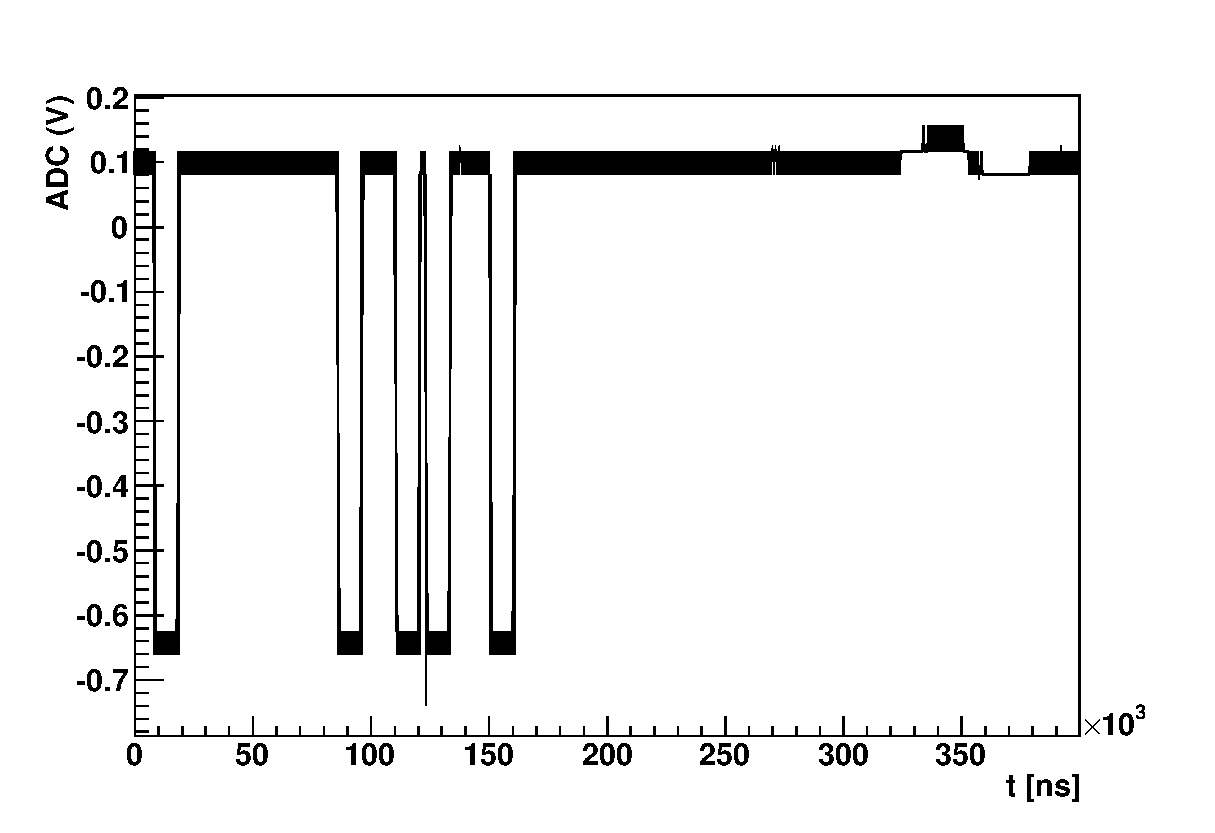
\includegraphics[width=0.9\textwidth]{MuonVetoExample}
						\caption[Example of the digitized muon veto channel.]
						{Example of the digitized muon veto channel, the low signal indicates a veto fire.}
						\label{fig:MuonVetoExample}
					\end{figure}
					\begin{lstlisting}
class MGMMuonVeto: public TObject
{
  public:
    std::vector<MGWaveformRegion> regions;
    bool IsInVetoRegion(size_t);
    bool RangeIsInVetoRegion(size_t beginning, size_t end);
  public:
    size_t GetNumberOfRegions() { return regions.size(); }
    
  ClassDef(MGMMuonVeto,1)
};
					\end{lstlisting}		
			\subsubsection{Modified-\bege~Tier0\texorpdfstring{$\to$}{ to }Tier1 Analysis}	
The analysis script for the modified-\bege~is unfortunately too long to reproduce here, but is freely available online at:
\url{http://github.com/mgmarino/BeGeAnalysisClasses/blob/master/BEGeAnalyzeWaveforms/analyze_waveforms.py}.  This 
script made extensive use of MGDO classes as well as the container classes described above and is provided as a reference
for using MGDO in production.
					
	\section{Analysis Database and Processing Framework}
	\label{sec:AnalysisDBProcFramework}
	The analysis database was set up to facilitate the movement and analysis of
data from beginning of processing (data acquisition) to the end (exclusion
plots, physics analyses, etc.).  The database ran using a \couchdb~backend, a
document-based database with several desirable features, including scalability
using the `view' Map-Reduce functionality and simple backup and mirror
propagation through built-in replication.  Replication allows quick and easy
distribution of data to several servers, very desirable for collaborations
wishing to share or mirror data in multiple locations.  As well, the \couchdb~server employs a RESTful interface, accepting basic http commands to access and
manipulate data and distributing and storing data in a JSON (JavaScript Object
Notation) format.  This interface simplifies communication with the database
server and has fostered the development of \couchdb~`wrappings' in several
languages including Ruby and Python.  More information on this database can be
found online at~\url{http://couchdb.apache.org/}.  This section will describe
the basic functionality of the run/analysis database as well as describe
particular details of its implementation.  

		\subsection{Overview}
		
	The central \couchdb~server for the run/analysis database was located on a
machine at the University of Washington and backed up to several other
instances including personal laptops and online at CloudAnt
(\url{https://cloudant.com/}).  The code written to encapsulate and read
out/run the database was written in Python using an older version of
couchdb-python (available \url{http://code.google.com/p/couchdb-python/}).
Other software with \couchdb~Python `bindings' is available including couchdbkit
(\url{http://couchdbkit.org/}), but the former was initially chosen for
arbitrary reasons.  The functionality of both frameworks is similar and so a
translation from one to the other should not entail a significant amount of
effort.  Three databases were run with this code, one for each of three
different detectors: \ppc1, \ppc2, and the low-background modified-\bege~detector.  \ppc2
and the modified-\bege~are described previously in this dissertation.  The code is freely
available in a browsable git repository online at:
\url{http://github.com/mgmarino/SoudanDB}.  			

			\lstset{language=sh}
			\begin{itemize}
		  	  	\setlength{\itemsep}{0.5pt}
		  	  	\setlength{\parskip}{0pt}
		  	  	\setlength{\parsep}{0pt}
				\item[] \lstinline!management! -- sub-module for management objects 
				\item[] \lstinline!utilities! -- sub-module for utility functions 
				\item[] \lstinline!update! -- sub-module housing objects for updating the database 
				\item[] \lstinline!views! -- sub-module housing objects and base classes for database views 
				\item[] \lstinline!databases! -- sub-module housing database objects 
				\begin{itemize}
		  	  		\setlength{\itemsep}{0.5pt}
		  	  		\setlength{\parskip}{0pt}
		  	  		\setlength{\parsep}{0pt}
					\item[] \lstinline!bege_gretina! -- Database for Gretina DAQ readout of the modified \bege
					\item[] \lstinline!bege_jc! -- Database for NI DAQ readout of the modified \bege~(see Section~\ref{sec:BeGeExperimentalSetup}) 
					\item[] \lstinline!ppctwo! -- Database for test stand readout of \ppc1 (not described in this dissertation 
				\end{itemize}
			\end{itemize}
The \lstinline!database! directories each had the following sub-structure with relevant code for the particular database:
			\begin{itemize}
		  	  	\setlength{\itemsep}{0.5pt}
		  	  	\setlength{\parskip}{0pt}
		  	  	\setlength{\parsep}{0pt}
				\item[] \lstinline!db.py! -- module providing particular code for the database 
				\item[] \lstinline!views! -- module providing separate Python files for each view 
				\item[] \lstinline!update! -- module providing separate Python files for each update function 
			\end{itemize}
	
Instead of describing the code in
depth, the following sections will focus on key functional aspects of the
database as they pertain to the creation of future databases.  

		\subsection{Functional Overview}
		
	The purpose of the run/analysis database was to track run information and
data and manage the analysis process.  A schematic of this process is shown in
Figure~\ref{fig:RunDBSchem}.  Metadata (e.g.~names of run files, time
information, parameter settings, etc.) generated by the DAQ system or slow
controls is automatically inserted into the database as a record when a new run
file is generated or run settings are changed.  Once this information appears
in the database, a process management class can then determine what types of
processing needs to happen to the metadata record and then execute the
necessary tasks to complete these.  In the schematic in
Figure~\ref{fig:RunDBSchem}, the process management class queries the run
database to determine which records have associated data that still requires
back up or analysis processing and then calls the associated program(s) to
complete this.  This methodology can scale well to larger numbers of data
records since processing (e.g.~cpu usage) only occurs when needed.  

			\begin{figure}
				\centering
				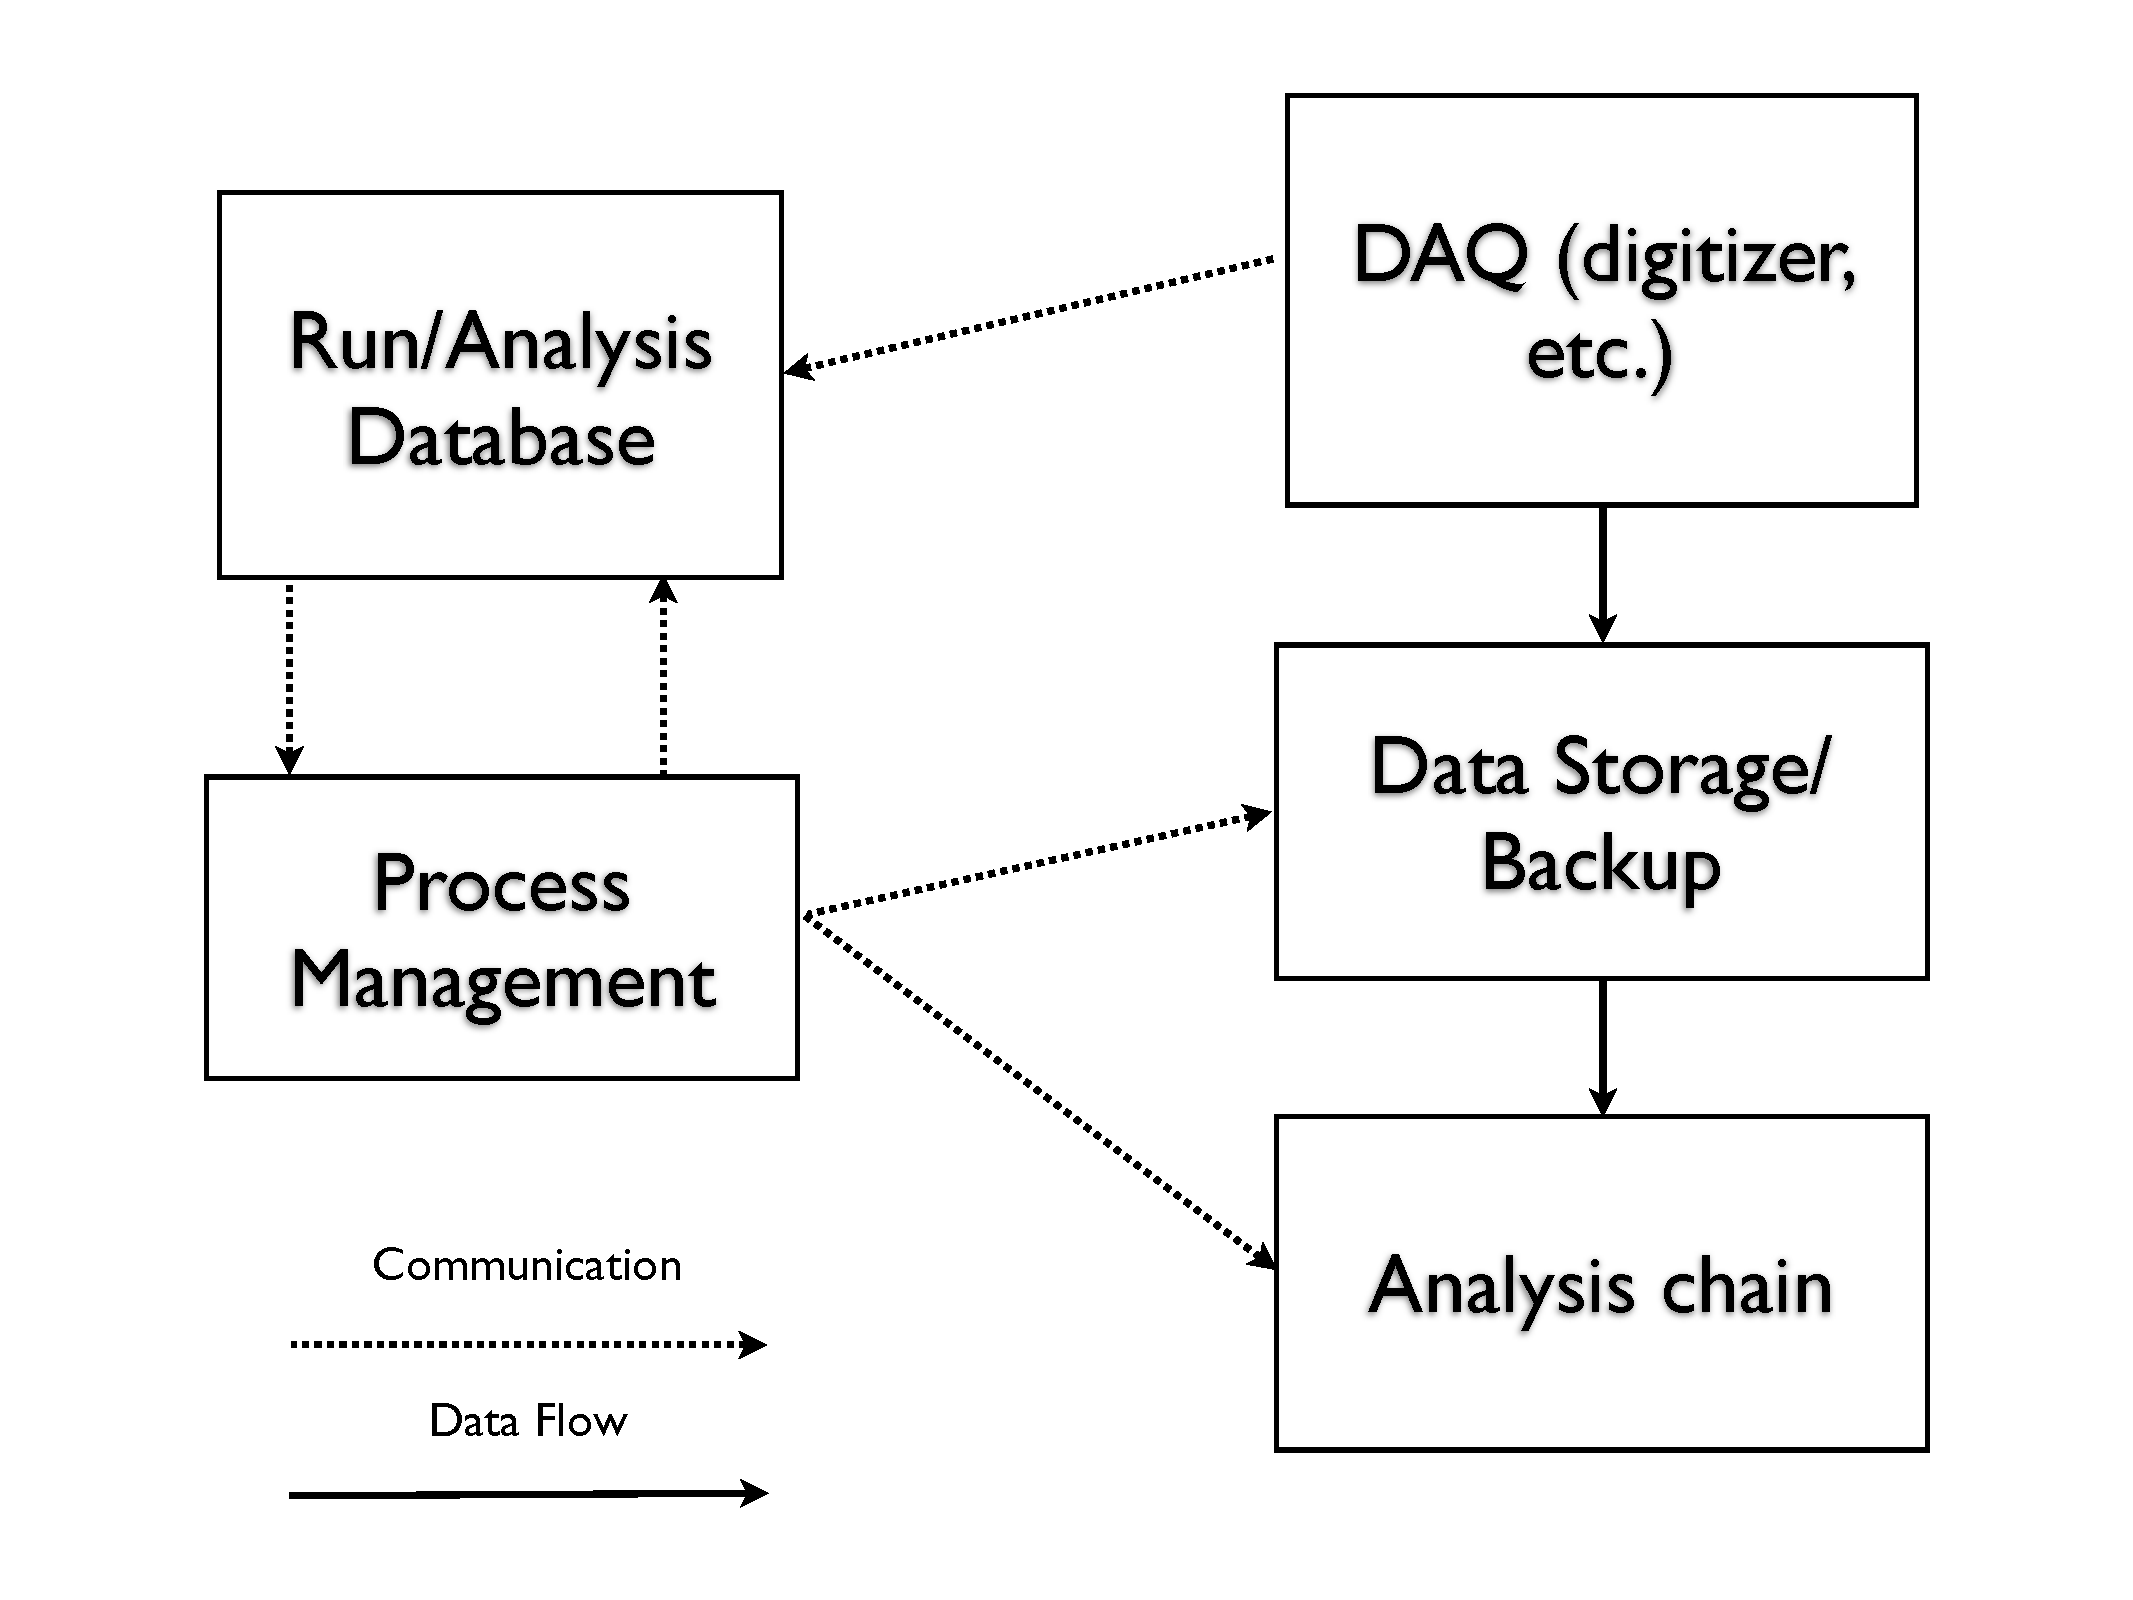
\includegraphics[width=0.7\textwidth]{RunDatabaseSchematic}
				\caption[Schematic of the run/analysis database functionality.]
				{Schematic of the run/analysis database functionality.}
				\label{fig:RunDBSchem}
			\end{figure}	

	Another advantage of using a \couchdb~database is that it is possible to insert records with different internal structure or different
metadata.  For example, a single database can include records of associated run metadata as well as other records with slow control information.  Additionally, metadata need not be consistent across records of a certain type.  This has the advantage that it is not required to fully define the data structure within a database during initial deployment, therefore allowing simple adaptability to any changes that will inevitably happen to the data-taking process such as adding a new channel or additional sets of information.  

		\subsection{Functional Implementation}
			\lstset{
		   language=JSON,
		   %backgroundcolor=\color{lightgray},
		   extendedchars=true,
		   basicstyle=\footnotesize\ttfamily,
		   showstringspaces=false,
		   showspaces=false,
		   numbers=left,
		   numberstyle=\footnotesize,
		   numbersep=9pt,
		   tabsize=2,
		   breaklines=true,
		   showtabs=false,
		   captionpos=b}	

	Implementing the functionality described in the previous section involved
taking advantage of several features built into the \couchdb~database.  The
database update could occur via several methods, for example: a daemon which
runs regularly to insert the metadata when new files or information from the
DAQ are generated; a system interrupt process calling an insertion function or
program when a new file appears in a certain directory; active insertion
(direct communication) by the DAQ software into the database.  This software
employed the first method, regularly running a daemon via a cron job to
determine when a new file was written into a certain directory by the DAQ
software and inserting the necessary metadata as a record into the database.  
	
	The initial insertion of metadata placed a skeleton record in the database,
populating the fields of the record with available data and leaving other
fields that required information from further processing empty.  The data
resided in the database in JSON format, and an example of a portion of an
inserted JSON record in the run/analysis database is shown in
Listing~\ref{lst:JSONExample}.  In this example, one can see the left-empty
fields denoted by {\ttfamily null}.  It is simple to write a `view' (a \couchdb~query) to return records where an empty field might exist.  This method can be
used to select records for processing.  For example, in the record snippet,
thet \lstinline!root_data_file_tier_1! has daughter values set to
\lstinline!null! including \lstinline!last_mod_time! (last modification time)
and \lstinline!md5hash! (calculated md5 hash) indicating that this particular
file in the analysis chain has yet to be created.  The process management
daemon could then run the proper program or function to generate this file and
populate those fields.  Other fields with \lstinline!null! also require some
further processing.  
	

			\begin{lstlisting}[caption=Truncated example of a JSON record in the run/analysis database., label=lst:JSONExample]
{
   "_id": "20100713120006",
   "_rev": "6-8ba079fbf9a7196c83b14aaf9976678b",
   "modification_time": null,
   "raw_data_file_tier_0": {
       "last_mod_time": "2010-07-13T12:22:07Z",
       "lfn": "tier0/100713120006",
       "md5hash": "c669edfa8e5a671b0a7c4e84932decb1",
       "pfn": "/data/Soudan/Data/BeGe/tier0/100713120006"
   },
   "number_of_entries_in_tier1_root_tree": null,
   "quality_assurance": {
       "qa_check_process_has_been_run": null,
       "qa_accept_run": null
   },
   "livetime": {
       "run_milliseconds": 9046984,
       "run_milliseconds_error": 0
   },
   "local_time_of_start_of_run": "2010-07-13T12:00:06Z",
   "root_data_file_tier_1": {
       "last_mod_time": null,
       "lfn": "tier1/100713120006_rootified.root",
       "md5hash": null,
       "pfn": "/data/Soudan/Data/BeGe/tier1/100713120006_rootified.root"
   },
   "run_settings": [
       "8000",
       "20000000",
       "20"
   ],
   ...
}
			\end{lstlisting}	

			\lstset{language=Python}		
	In the database sub-modules, the framework associates `views' with
processing functions in the `update' module.  This allows updates to be
performed on records returned by particular views.  Each update module
(e.g.~\lstinline!SoudanDB.databases.bege_jc.update.update_number_of_entries_in_root_file!)
exports two functions: \lstinline!get_view()! and \lstinline!update_rundoc(run_doc)!.  Therefore,
a daemon management program would use the \lstinline!get_view()! to return the records needing
updates and then run \lstinline!update_rundoc()! for each \lstinline!run_doc!.  The management process
for doing this is located in \lstinline!SoudanDB.update.update_calculations_on_database!.
Newer versions of \couchdb~should allow such processing to occur within the
view server framework of the database itself.  For example, the \couchdb~server should eventually be
able to handle both generating the views and running the update functions on
those views.  Therefore, future implementations should not use this daemon
methodology and instead should migrate to using a Python view server.  

		
	\section{WIMP PDFs Software Framework}
	\label{sec:WIMPPDFs}
	% Discussing pyWIMP.  Touch on the most useful features, in particular the WIMPPds and DMModel
	This section outlines and describes the functionality of the pyWIMP software package for generating fits and limits
to dark matter interactions such as a WIMP-nuclear recoil or the axioelectric effect.  The software is freely available in a 
git repository online at \url{http://github.com/mgmarino/pyWIMP}.  The software is written as a Python/\cpp~hybrid package, essentially
using Python for process control and management and using compiled \cpp~code where speed is critical.  As with most work performed for a thesis, some significant effort was placed in the initial design and development of this package, but as deadlines approached and the pressure to make it just \emph{work} increased, some code not generally useful necessarily appeared.  Because of this, the following sections will discuss the code that \emph{is} generally useful in the hopes that its development will save the same effort from others.  
	
		\subsection{Overview}
	The pyWIMP package makes extensive use of the RooFit fitting package~\cite{ver03aa} -- developed for BaBar and now included in the ROOT analysis package~\cite{Bru97}.  The basic structure of pyWIMP is as follows:
	
			\lstset{language=sh}
			\begin{itemize}
		  	  	\setlength{\itemsep}{0.5pt}
		  	  	\setlength{\parskip}{0pt}
		  	  	\setlength{\parsep}{0pt}
				\item[] \lstinline!buildTools/! -- directory for building utilities
				\item[] \lstinline!test_scripts/! -- directory containing test scripts useful for checking for proper installation
				\item[] \lstinline!pyWIMP/! -- base directory of Python package
				\begin{itemize}
		  	  		\setlength{\itemsep}{0.5pt}
		  	  		\setlength{\parskip}{0pt}
		  	  		\setlength{\parsep}{0pt}
					\item[] \lstinline!Calculation! -- sub-module containing Python calculation classes for deriving sensitivities and limits
					\item[] \lstinline!DMModel! -- sub-module containing Python objects for the construction of models used in fitting dark matter signals
					\item[] \lstinline!WIMPPdfs! -- sub-module containing compiled \cpp~classes used to construct dark matter signal models
					\item[] \lstinline!utilities! -- utilities sub-module
				\end{itemize}
			\end{itemize}
Since the most generically useful tools exist in the WIMPPdfs and DMModels sub-modules, the following sections will detail these.
			\lstset{language=Python}		
		\subsection{\texorpdfstring{\lstinline!pyWIMP.WIMPPdfs!}{pyWIMP.WIMPPdfs}}
			\lstset{
			   language=C++,
			   backgroundcolor=\color{white},
			   extendedchars=true,
			   basicstyle=\footnotesize\ttfamily,
			   %keywordstyle=\bfseries,
			   showstringspaces=false,
			   showspaces=false,
			   numbers=none,
			   numberstyle=\footnotesize,
			   numbersep=9pt,
			   tabsize=2,
			   breaklines=true,
			   showtabs=false,
			   captionpos=t}

WIMPPdfs contains \cpp-constructed objects of probability distribution functions and related classes.  Almost all of the classes derive from \lstinline!RooAbsPdf!, except for classes used for Form Factor calculation which derive from \lstinline!MGMVWimpFormFactor!.  All classes are described in detail here, including their functionality and primary constructor.  
			\paragraph{\lstinline!class MGMVWimpFormFactor!}
Base class for all classes describing a form factor.  This class has a standard constructor, but should never need to be directly
instantiated by a user: 
				\begin{lstlisting}
MGMVWimpFormFactor(const char *name = "", const char *title = "")
				\end{lstlisting}			
				
			\paragraph{\lstinline!class MGMWimpHelmFFSquared!}
Class describing a Helm nuclear form factor squared~\cite{Helm56}, the default constructor is: 
				\begin{lstlisting}
MGMWimpHelmFFSquared(const char *name, const char *title, 
	RooAbsReal& _q, 
	RooAbsReal& _r_sub_n, 
	RooAbsReal& _s)
				\end{lstlisting}
where \lstinline!_q! is the momentum transfer, \lstinline!_r_sub_n! is the effective nuclear radius and \lstinline!_s! is the skin thickness.
			
			\paragraph{\lstinline!class MGMBetaDecayFunction!}
Class describing a generic beta decay.  This class does not take into account any correction factors and instead gives the kinematic spectrum for the electron given the endpoint energy of the decay.  The default constructor is			
				\begin{lstlisting}
MGMBetaDecayFunction(const char *name, const char *title,
	RooAbsReal& _energy,
	RooAbsReal& _mass_of_electron,
	RooAbsReal& _qvalue)
				\end{lstlisting}	
where \lstinline!_enery! is the energy of the electron, \lstinline!_mass_of_electron! is the mass of the electron and  \lstinline!_qvalue! is the q-value of the decay, all in keV.

			\paragraph{\lstinline!class MGMErfcFunction!}
Class implementing an error function pdf of the form: $ \frac{1}{2}\operatorname{erf} ((E-\mu)/(\sigma \sqrt{2})) + \rho$ with $\rho$ the offset.  The constructor:
				\begin{lstlisting}
MGMErfcFunction(const char *name, const char *title,
	RooAbsReal& _energy,
	RooAbsReal& _mean,
	RooAbsReal& _sigma,
	RooAbsReal& _offset)
				\end{lstlisting}			
				
			\paragraph{\lstinline!class MGMWimpDiffRateBasicPdf!}
Class implementing the basic form of the WIMP interaction with no time dependence~\cite{Lew96}: $0.751 R_{0}/(E_{0} r) \exp(-0.561 \frac{Q}{E_{0} r })$
				\begin{lstlisting}
MGMWimpDiffRateBasicPdf(const char *name, const char *title,
	RooAbsReal& _R_sub_0,
	RooAbsReal& _E_sub_0,
	RooAbsReal& _Q,
	RooAbsReal& _r,
	MGMVWimpFormFactor& _form_factor = MGMVWimpFormFactor::DefaultFormFactor())
				\end{lstlisting}	

			\paragraph{\lstinline!class MGMWimpDiffRatePdf!}
Class implementing the time-dependent WIMP interaction assuming infinite escape velocity (see Section~\ref{sec:CalcLimitsOnWIMPSignal} and~\cite{Jun96,Lew96}), where $v_{E}$ is the velocity of the earth with possible time dependence.  This class takes advantage of RooFit functionality which does not require parameters to have explicit dependencies.  That is, this class does not need to know about any time dependence of $v_{E}$.
				\begin{lstlisting}
MGMWimpDiffRatePdf(const char *name, const char *title,
	RooAbsReal& _v_sub_0,
	RooAbsReal& _v_sub_min,
	RooAbsReal& _v_sub_E,
	RooAbsReal& _R_sub_0,
	RooAbsReal& _E_sub_0,
	RooAbsReal& _r,
	MGMVWimpFormFactor& _form_factor = MGMVWimpFormFactor::DefaultFormFactor())
				\end{lstlisting}	
						
			\paragraph{\lstinline!class MGMWimpDiffRateEscapeVelPdf!}
Class implementing the time-dependent WIMP interaction with the finite escape velocity of the dark matter halo included.  This class is equivalent to the above class with the addition of the the escape velocity parameter, $v_{\text{esc}}$.  See Section~\ref{sec:CalcLimitsOnWIMPSignal} for details on the functional form of this pdf.
				\begin{lstlisting}
MGMWimpDiffRateEscapeVelPdf(const char *name, const char *title,
	RooAbsReal& _v_sub_0,
	RooAbsReal& _v_sub_min,
	RooAbsReal& _v_sub_E,
	RooAbsReal& _R_sub_0,
	RooAbsReal& _E_sub_0,
	RooAbsReal& _r,
	RooAbsReal& _v_sub_esc,
	MGMVWimpFormFactor& _form_factor = MGMVWimpFormFactor::DefaultFormFactor());
				\end{lstlisting}	

			\paragraph{\lstinline!class MGMWimpTimeFunction!}
Class implementing a generic time pdf for a WIMP search with the functional form: $v_{0} + v_{1}\sin{2\pi t}$.  This is useful for deriving sensitivity or looking for limits on a generic oscillation signal.			
				\begin{lstlisting}
MGMWimpTimeFunction(const char *name, const char *title,
	RooAbsReal& _velocity_0,
	RooAbsReal& _velocity_1,
	RooAbsReal& _time);

				\end{lstlisting}
					
			\lstset{
			   language=Python}							
		\subsection{\texorpdfstring{\lstinline!pyWIMP.DMModels!}{pyWIMP.DMModels}}
		
	DMModels provides a sub-module of Python objects that return generically
useful PDFs.  The purpose of this module is to provide simple objects with
interfaces to derive PDFs for sensitivity and limit calculations.  Base classes
are defined in \lstinline!DMModels.base_model!, which are used by other Python
objects in this sub-module.  All of the model classes have a \lstinline!get_model()!
routine which returns a RooAbsPdf.  Some model classes may return other PDFs; those 
are indicated where applicable.
	
			\paragraph{\lstinline!DMModels.base_model!}
Defines \lstinline!DMModels.base_model.BaseVariables! and
\lstinline!DMModels.base_model.BaseModel!.  The first provides an encapsulation
class for the observables time (in years) and energy (in keV) and the second
provides a base class for other objects in this submodule.
\lstinline!DMModels.base_model.BaseVariables! can be instantiated by:
				\begin{lstlisting}			
base_variabes =  DMModels.base_model.BaseVariables( 
                 time_beginning,   # Define the beginning of time obs
                 time_in_years,    # Define the end of time observation
                 energy_threshold, # Energy threshold (keV)
                 energy_max,       # Maximum energy range (keV)
                 use_tag = True    # Use a tag, useful when using 
                                   # multiple instances of this class.
                 ) 
				\end{lstlisting}				

			\paragraph{\lstinline!DMModels.beta_decay_model!}
Defines \lstinline!DMModels.beta_decay_model.BetaDecalModel! which generates the kinematic
electron spectrum of a beta decay.  Also, if the lifetime of the decay is included, the returned PDF will
be 2-D in energy and time.  In can be instiated by 
				\begin{lstlisting}			
beta_decay =     DMModels.beta_decay_model.BetaDecalModel(
                 base_variabes,   # Base variables (BaseVariables class), 
                 q_value,         # Q value of the beta decay (float)
                 lifetime = None  # Lifetime (in years, float), if None 
                                  # then the returned PDF is flat in time
                 )
beta_decay_model = beta_decay.get_model() # Return the RooAbsPdf
				\end{lstlisting}				

			\paragraph{\lstinline!DMModels.tritium_decay_model!}			
Defines \lstinline!DMModels.tritium_decay_model.TritiumDecayModel! which generates the kinematic decay of
tritium.  This class returns a 2-D tritium decay spectrum with an additional flat background.  
It returns an extended model with the relative amounts are set correctly (but allowed to float)
This means that if you are doing toy model fitting with the returned model before to generate
the events (RooFit will automatically generate the correct number of events from an extended pdf)
and SAVE all the variables. 

				\begin{lstlisting}			
tritium_decay =  DMModels.tritium_decay_model.TritiumDecayModel(
                 base_variables,     
                 tritium_exposure,    # Tritium Exposure time (days) 
                 tritium_activation,  # Tritium activation rate 
                                      # in atoms/kg/day 
                 mass_of_detector,    # Mass of the detector (kg)
                 flat_background_rate # Flat background rate, 
                                      # in counts/kg/keV/day
                 )
tritium_model = tritium_decay.get_model() # Return RooExtendPdf
				\end{lstlisting}				

			\paragraph{\lstinline!DMModels.flat_model!}
Defines \lstinline!DMModels.flat_decay_model.FlatModel! which generates a pdf flat in both time and energy. 

				\begin{lstlisting}			
flat =           DMModels.falt_decay_model.FlatModel(
                 base_variables)     
flat_model = flat.get_model() # Return RooAbsPdf
				\end{lstlisting}				

			\paragraph{\lstinline!DMModels.gamma_line_model!}
Defines \lstinline!DMModels.gamma_line_model.GammaLineModel! and \lstinline!DMModels.gamma_line_model.GammaLineFactory!.  The
first defines a basic object to handle a gamma (or x-ray line) at a certain energy and a defined sigma.  The second is a 
convenience class to limit the generation of code when implementing a gamma line. 
				\begin{lstlisting}			
gamma =          DMModels.gamma_line_model.GammaLineModel(
                 base_variables,
                 mean,            # Mean, RooAbsReal
                 sigma,           # Sigma, RooAbsReal
                 lifetime = None  # Lifetime, float, if None, 
                                  # return PDF is 1-D
                 )
gamma_model = gamma.get_model()
				\end{lstlisting}				
The factory includes two convenience functions to quickly return a gamma line:
				\begin{lstlisting}			
gamma =          DMModels.gamma_line_model.GammaLineFactory.generate(
                 mean,           # Mean, float
                 lifetime,       # Lifetime, float
                 base_variables)
gamma_model = gamma.get_model()
# ... OR alternatively explicitly define errors ...
gamma =          DMModels.gamma_line_model.GammaLineFactory.generate(
                 mean,           # Mean, float
                 mean_error,     # Mean error, float
                 sigma,          # Sigma, float
                 sigma_error,    # Sigma error, float
                 lifetime,       # Lifetime, float
                 base_variables)
gamma_model = gamma.get_model()

				\end{lstlisting}				

			\paragraph{\lstinline!DMModels.wimp_model!}	
Defines \lstinline!DMModels.wimp_model.WIMPModel! which is a class wrapping several different WIMP PDFs.  At the time
of writing, the class was tuned to work with germanium detectors as it included quenching and atomic information
specific to a germanium detector.  Modifying the class to be applicable to other detectors should not be difficult.  
The models that this class returns require a normalization factor, which is the \emph{nuclear}
cross section of the WIMP interaction (i.e.~not normalized per nucleon).  
Therefore, all classes should use a \lstinline!RooExtendPdf! to multiply the cross-section by the obtained \lstinline!RooAbsPdf!.  
The class is instantiated:
				\begin{lstlisting}			
wimp_class =     DMModels.wimp_model.WIMPModel(
                 base_variables, 
                 mass_of_wimp,      # Mass of the WIMP (GeV) 
                 kilograms,         # Mass of the detector (kg)
                 constant_quenching # If true, use constant, non-energy 
                                    # dependent quenching
                                    # Else use energy-dependent quenching.
                 )
# Get normalization: multiply cross-section by this to get 
# per-nucleon xs (in pb ) (returns RooRealVar)
wimp_nucleon_norm = wimp_class.get_normalization() 

# Get simple (only 1-D exponential) model (returns RooAbsPdf)
wimp_simple = wimp_class.get_simple_model()        

# Get different form factors (returns RooAbsPdf)
helm_ff = wimp_class.get_helm_form_factor()
exponential_ff = wimp_class.get_exponential_form_factor()

# Get different 2-D WIMP models.  The following allow
# changing the value of the WIMP mass by passing
# in an (optional) float parameter

wimp_model_no_escape_velocity = \
    wimp_class.get_WIMP_model(20) # Change mass to 20
# WIMP Model, escape velocity, form factor = 1
wimp_model_esc_vel_no_ff = \
    wimp_class.get_WIMP_model_with_escape_vel_no_ff()

# WIMP Model, escape velocity, Helm form factor
wimp_model = wimp_class.get_WIMP_model_with_escape_vel()
# ... OR equivalently ... 
wimp_model = wimp_class.get_model()

				\end{lstlisting}				

		\subsection{Calculating Sensitivities}
The \lstinline!pyWIMP! package includes a utility executable, \lstinline!job_engine.py!, that can distribute
many different calculations across several CPUs.  (There are also several examples of using this sofware package
with MPI using the Python mpi4py distribution.  These can be found in e.g.~in \lstinline!test_Rolke.py, mpi_job_engine.py!, 
but the usage of this is not detailed here.)  This executable may be called with several different options, which are presented
here for reference:

				\lstset{language=csh, tabsize=4}
				\begin{lstlisting}	
> python /path/to/pyWIMP/job_engine.py WIMPModel --help
Usage: job_engine.py model [options]

Options:

  -h, --help            show this help message and exit
  --total_time=TOTAL_TIME
                        Total time (year)
  --print_out_plots     Print plot results of fit to eps format.   This will
                        cause the program to continue instead of stopping once
                        a plot is made. Batch mode will be set so that no plot
                        will be displayed during the program.
  --tritium_activation_rate=TRITIUM_ACTIVATION_RATE
                        Tritium activation rate (counts/kg/day)
  --constant_energy     Set energy as constant
  --do_axioelectric     Do axioelectric fitting
  --wimp_mass=WIMP_MASS
                        WIMP mass (GeV/c^-2)
  --num_time_bins=NUM_TIME_BINS
                        Number of time bins, 0 means unbinned
  --energy_max=ENERGY_MAX
                        Maximum energy (keV)
  --num_energy_bins=NUM_ENERGY_BINS
                        Number of energy bins, 0 means unbinned
  --debug               Set debug flag, enables verbose output
  --axion_mass=AXION_MASS
                        Axion mass in keV [default 0]
  --constant_time       Set time as constant
  --variable_quenching  Set to use variable quenching
  --threshold=THRESHOLD
                        Threshold (keV)
  --tritium_exposure_time=TRITIUM_EXPOSURE_TIME
                        Tritium exposure time days
  --confidence_level=CONFIDENCE_LEVEL
                        Confidence level (0 -> 1)
  --show_plots          Show plot results of fit
  --background_rate=BACKGROUND_RATE
                        Background rate (counts/keV/kg/day)
  --mass_of_detector=MASS_OF_DETECTOR
                        Mass of detector (kg)
  -o OUTPUT_FILE, --output_file=OUTPUT_FILE
                        Define the output file name (full path)
  -n NUMPROCESSORS, --num_cpus=NUMPROCESSORS
                        Define the number of cpus used
  -a MAX_TIME, --max_time=MAX_TIME
                        Set the max time [seconds] until this program shuts
                        down
  -i NUM_ITER, --num_iter=NUM_ITER
                        Number of iterations per cpu
				\end{lstlisting}	

For example, to perform a sensitivity calculation on a WIMP mass of 20~GeV, with a \MJ-like detector
of 20~kg over 5~years, one could execute:
				\begin{lstlisting}
/path/to/pyWIMP/job_engine.py WIMPModel	\
  -o output_root_file.root 				\
  -n 8 									\
  -i 1000 								\
  --mass_of_detector=20 				\
  --wimp_mass=20 						\
  --tritium_exposure_time=30			\
  --tritium_activation_rate=200			\
  --total_time=5 						\
  --background_rate=0.001 				\
  --energy_max=20 						\
  --threshold=0.5 						\ 
  --confidence_level=0.9 				\
				\end{lstlisting}
which would distribute the workload across 8~cpus.  Similarly, to calculate the sensitivity to an axioelectric effect at an axion
mass of 3~keV, one might use the additional flags:
				\begin{lstlisting}
  --do_axioelectric						\
  --axion_mass=3 						\
				\end{lstlisting}
and drop the flag \lstinline!--wimp_mass!.  

Currently, limit calculations on data can also be performed using \lstinline!`job_engine.py DataExclusion`!, but this is currently limited
to a background model consistent with that from the modified-\bege~detector described in Section~\ref{sec:LimitsDataAndModel}.  Therefore, any application of this framework to other data sets would require the construction of a background model to suitably 
describe that dataset.  It is the hope that this toolkit together with the tools already available in RooFit would provide
everything necessary for building such a model.
